\documentclass[times,11pt]{article}
\newcommand{\nop}[1]{}
\newcommand\ASI{{\it ASI}}
\usepackage{wrapfig}
\usepackage{mathrsfs}
%\usepackage{psfig}
\usepackage{epsfig}
\usepackage{graphics}
\usepackage{epsf}
\usepackage{amsmath, amsthm, amssymb, multirow, paralist, subfigure}
\usepackage{fullpage}
\usepackage{url,color}
\usepackage{algorithm,algorithmic}
\usepackage{epstopdf}
\newtheorem{thm}{Theorem}
\newtheorem{prop}{Proposition}
\newtheorem{lemma}{Lemma}
\newtheorem{cor}[thm]{Corollary}
\newtheorem{definition}[thm]{Definition}

\def \B {\mathcal{B}}
\def \x {\mathbf{x}}
\def \H {\mathcal{H}_{\kappa}}
\def \R {\mathbb{R}}
\def \w {\mathbf{w}}
\def \wh {\widehat{\w}}
\def \sgn {\mbox{sgn}}
\def \a {\mathbf{a}}
\def \u {\mathbf{u}}
\def \uh {\widehat{\u}}
\def \wt {\widetilde{\w}}
\def \E {\mathrm{E}}
\def \C {\mathcal{C}}
\def \xh {\widehat{\x}}
\def \xt {\widetilde{\x}}
\def \yh {\widehat{y}}
\def \A {\mathcal{A}}
\def \S {\mathcal{S}}
\def \Mh {\widehat{M}}
\def \Z {\mathcal{Z}}
\def \xt {\widetilde{\x}}
\def \Xh {\widehat{X}}
\def \D {\mathcal{D}}
\def \z {\mathcal{z}}
\def \h {\mathbf{h}}
\def \c {\mathbf{c}}
\def \z {\mathbf{z}}
\def \sh {\widehat{s}}

%\usepackage{fullpage,comment,times}
%\usepackage{graphicx}
%\usepackage{subfigure}
%\usepackage{wrapfig}
%\usepackage{cite}
%    \ifx\pdfpagewidth\undefined\else\pdfpagewidth 8.5in\fi
%    \ifx\pdfpageheight\undefined\else\pdfpageheight 11in\fi


\begin{document}

\title{Modeling Plant Photosynthesis Heterogeneity under Dynamic Light Conditions}

\author{Oliver Tessmer, Jeff Cruz, David M Kramer, Jin Chen}

\maketitle

\section{Introduction}

With the advent of models for biomedical image analysis, heterogeneity, a concept relating to the uniformity in a substance, has assumed new importance since last decade (Tiihonen 1997; Wieneke 1999, Wang 2000). In plant biology, photosynthetic heterogeneity refers to a plant comprising multiple regions, many of which have different photosynthesis properties, potentially because of vastly different $CO_2$ intake capability, stomatal conductance and tolerance level to environmental changes.

Photosynthetic heterogeneity is a universal phenomenon among plants (Charles 2008). With the rapid development of lighting and imaging techniques, real-time non-invasive monitoring of photosynthesis became feasible, resulting in vast amount of phenotype data (Wituszynskaa 2013). A consensus view of the data is that the photosynthesis ability of a plant is not uniform across the whole area (Charles 2008, Meng 2007). By integrating plant morphological and physiological features, measuring plant photosynthetic heterogeneity aids interpretation of the sophisticated phenotyping data, particularly important for plant primary productivity estimation and modeling (Meng 2007).

The granularity of photosynthetic heterogeneity of plants ranges from cells to tissues, leaves, and even the whole plant level. While in-leaf variability in photosynthetic activity has been well studied for the understanding of the effects of stomatal conductance \cite{Cheeseman1991,Buckley1997}, recent works show that photosynthetic capacity may decline with vertical gradient and leaf age, indicating that leaf-based photosynthetic heterogeneity is a key towards the understanding of plant total photosynthesis \cite{Kitajima2002,ChenCP2008}.

To measure leaf-based photosynthetic variability in a nowadays popular large-scale phenotyping experiment, in which hundreds of plants are monitored simultaneously in real time, it is naturally required to segment each leaf from top-view photosynthesis images automatically. Photosynthesis images are false-color images, where the light intensity of every pixel is proportional to photosynthetic efficiency (Toet 1996). Differences between individual leaves with similar photosynthetic efficiency can be subtle, making the boundaries between them is difficult to define and creating a significant challenge for subsequent shape analysis. The difficulty even arises when individual leaves overlap and occlude one another in these false-color images.

We have developed a new leaf segmentation approach called leafPH to identify leaves from photosynthesis images...


In this paper, we present a new computational approach to compute leafPH. Comparing with the existing approaches, our method is novel in the following ways:

1.	Our measure relies on a new leaf segmentation method, which considers plant-specific constraints including leaf shape similarity and symmetry. By taking the biological knowledge about the shapes of any possible leaf into account, we add flexibility to the model to fit to all the general leaves. Specifically, for leaf boundary identification, we develop a leaf symmetry based curve fitting model to define the initial shape of a leaf, and develop a plant layout based approach to define leaf tips and orientation, therefore defining the leaf initial position.  Note that since leaf is assumed to be symmetric, curve fitting could converge without large amount of training.

2. Mathematically, leafPH refers to the differences between individual leaf photosynthesis and the pooled photosynthesis across all the leaves, with the weights being those used in the pooling method. With leafPH, transient regional variation events which do not affect the whole plant photosynthesis, can be easily discovered.

%---------------------------



\section{Background of heterogeneity measurement}

The classical measure of heterogeneity is Cochran�s Q-test (Conover1999), which is calculated as the weighted sum of squared differences between individual study effects and the pooled effect across studies with the weights being those used in the pooling method. Q is distributed as a chi-square statistic with $k-1$ degrees of freedom, where $k$ is the number of studies, and each study is a comparison between observation and reference.

Q has low power as a comprehensive test of heterogeneity (Gavaghan et al, 2000), especially when the number of studies is small, i.e. most meta-analyses. Conversely, Q has too much power as a test of heterogeneity if the number of studies is large (Higgins et al. 2003): Q is included in each meta-analysis function because it forms part of the DerSimonian-Laird random effects pooling method (DerSimonian and Laird 1985). An additional test, due to Breslow and Day (1980), is provided with the odds ratio meta-analysis. It is arguably not possible to examine the null hypothesis that all studies are evaluating the same effect, by considering the only the summary data from the studies: The heterogeneity test results should be considered alongside a qualitative assessment of the combinability of studies in a systematic review.

The $I^2$ statistic (Higgins2003) describes the percentage of variation across studies that is due to heterogeneity rather than chance (Higgins and Thompson, 2002; Higgins et al., 2003). $I^2$ is an intuitive and simple expression of the inconsistency of studies� results. Unlike Q it does not inherently depend upon the number of studies considered. A confidence interval for $I^2$ is constructed using either i) the iterative non-central chi-squared distribution method of Hedges and Piggott (2001); or ii) the test-based method of Higgins and Thompson (2002). The non-central chi-square method is currently the method of choice (Higgins, personal communication, 2006) � it is computed if the 'exact' option is selected. The L'Abb� plot can be used to explore the inconsistency of studies visually.

To measure leaf-based photosynthetic variability in a large-scale phenotyping experiment, in which hundreds of plants are monitored in real time, it is naturally required to identify each leaf from top-view photosynthesis images automatically. However, leaf identification is a difficult task, in that 1) all the leaves are very similar in appearance especially for model plant Arabidopsis; 2) leaf features are much fewer than the well-studied face recognition problem; and 3) leaves may overlapped with each other that makes the problem more complicated. In short, there are two challenging computational problems. First, how to separate overlapped leaves in photosynthesis images where the leaf boundaries are obscure. Second, how to recognize incomplete leafs due to occlusion. Alternatively, approximation approaches can be used to estimate the leaf-based photosynthetic heterogeneity, including distribution based, region based and pixel based approaches. While these approximation approaches are easier to model, their performance may be reduced.

\section{Data Acquisition and Preprocessing}


In the photosynthesis phenotyping experiment, hundreds of Arabidopsis thaliana plants (wild type, genetic variations with gene knockout or over-expression, ecotypes, etc) were grown side-by-side under three different light conditions (constant, sinusoid, fluctuate), for in total three days.
%
Top-view fluorescence images were collected every 15 minutes in order to observe the photosynthesis activity of all of the plants simultaneously. Each fluorescence image is a grey-scale image with a resolution of 1M pixels at 12-bit intensity.

To accurately capture the photosynthesis activities of plants from fluorescence images, a image segment method is applied to remove the background, identify every piece of leaf~\cite{yin2014}, measure the intensity of pixels on leaves, and finally convert the intensity values to the measure of four kinds of photosynthesis parameters.
%
The extracted measurements of photosynthesis parameters are presented in the form of multi-dimensional time-series, one dimension for every photosynthesis parameter.
%
Figure 1 shows that the measurements of a photosynthesis parameter $\Phi_2$ at one time point are quite different for the leaves of the same plant  (i.e. plant no. 3-7 and 5-5).

\begin{wrapfigure}{r}{0.3\textwidth}
  \begin{center}
    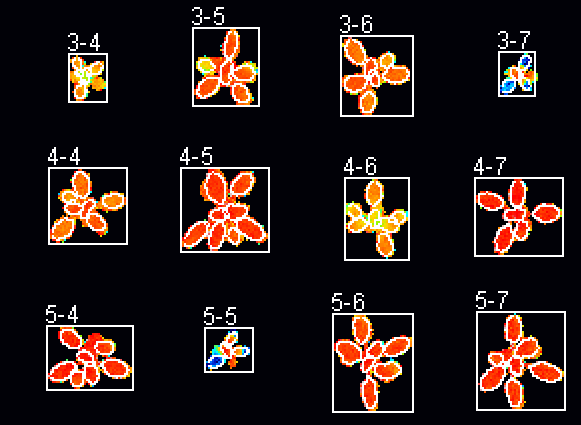
\includegraphics[width=0.3\textwidth]{preprocessing.png}
  \end{center}
  \caption{An example of leaf-level photosynthesis parameters in plants.}
  \label{fig:hardware}
\end{wrapfigure}

\section{Computing Photosynthesis Heterogeneity}

Heterogeneity is a concept relating to the uniformity in a substance (REF), which has assumed new importance since last decade with the advent of models for biomedical image analysis \cite{Tiihonen1997,Wieneke1999,Wang2000}. For example, heterogeneity in the aggressiveness of tumor cell populations has been adopted as an essential feature in predicting treatment success \cite{OSullivan2003}.

Photosynthetic heterogeneity refers to a plant comprising multiple regions, each of which has different photosynthesis efficiency, potentially because of vastly different tissues, sizes, developmental stages, and even transient variations over time.
%
Photosynthetic heterogeneity is a universal phenomenon among plants (REF). With the rapid development of lighting and imaging techniques, real-time non-invasive monitoring of photosynthesis became feasible, resulting in vast amount of data (REF). A consensus view of the data is that the photosynthesis ability of a plant is not the same (or similar) across the whole area (REF). By connecting plant morphological and physiological features, measuring photosynthesis heterogeneity aids interpretation of the sophisticated plant phenotyping data, in particular as evidence of consistency across studies.

%gap


\subsection{Leaf-based photosynthetic heterogeneity}

The traditional heterogeneity measure was designed to compute the differences between individual study effects, and for each individual study,  people assume only two underlying populations representing the
experimental vs. control groups on a continuous outcome. However, to compute the leaf-based photosynthetic heterogeneity, we have to compare all the leaves where each leaf may have its unique underlying population. To solve the more complicated problem, we modified the current Q test, and describe it in this section.

\subsubsection{Effect-size estimate for leaf pair-wise comparison}
%
Given a plant with $n$ leaves, we define a set $T = \{T_{11}, T_{12}, \ldots\}$, where $|T|=n\times(n-1)/2$, which is the total number of  pair-wise leaf-to-leaf comparisons. In each tuple $T_{ij}$, we compare the photosynthesis values of leaves $L_i$ and $L_j$ using Equation \ref{eq:T}.

\begin{equation}\label{eq:T}
T_{ij} = c(L_i, L_j) \frac{mean(L_i)-mean(L_j)}{S(L_i, L_j)}
\end{equation}

\noindent where $mean(L_i)$ is the averaged photosynthesis value of every pixel in leaf $L_i$, and $c(L_i, L_j)$ is a correction factor for the positive bias suffered by the standardized mean difference with small sample sizes, and can be estimated by $c(L_i, L_j) = 1-3/(4|L_i|+4|L_j|-9)$, according to (Hedges and Olkin 1985) \cite{hedges1998fixed}.
%
Such adjustment is necessary, because for small plants due to gene knockout, there may be only a few pixels for each leaf. According to the equation of $c(L_i, L_j)$, $c(L_i, L_j)$ is close to 1 for large leaves with many pixels, otherwise it is close to 0, downweighing the value of heterogeneity. $S$ is a pooled estimate of the within-group standard deviation using Equation \ref{eq:S} \cite{hedges1998fixed}.

\begin{equation}\label{eq:S}
S(L_i, L_j) = \sqrt{\frac{(|L_i|-1)std^2(L_i)+(|L_j|-1)std^2(L_j)}{|L_i|+|L_j|-2}}
\end{equation}

\noindent where $std^2(L_i)$ is the standard variance of leaf $L_i$ and $|L_i|$ is the total number of pixels in leaf $L_i$.

The sample variance of $T_{ij}$ is estimated using Equation \ref{eq:ST} \cite{hedges1998fixed}.

\begin{equation}\label{eq:ST}
ST_{ij} = \frac{|L_i|+|L_j|}{|L_i||L_j|}+\frac{T_{ij}^2}{2(|L_i|+|L_j|)}
\end{equation}

\subsubsection{Random effect-size estimate for all-leaf comparison}

Once an effect-size estimate is obtained from each pair-wise comparison, we integrate them by calculating an average effect size, assessing the statistical heterogeneity around the average estimate, and searching for moderator variables when there is more heterogeneity than can be explained by chance. In general, the most realistic statistical model to integrate the effect estimates in a meta-analysis is the
random-effects model, because it incorporates the two possible sources of heterogeneity among the studies, i.e., statistical variability caused by sampling error and substantive variability.

Given the set of all pair-wise comparisons $T$, we compute leaf-based photosynthetic heterogeneity LeafPH using Equation \ref{eq:LeafPH}.

\begin{equation}\label{eq:LeafPH}
LeafPH = \frac{\sum_{i,j} w_{ij}(T_{ij}-\bar{T})}{|T|}
\end{equation}

\noindent where $\bar{T}$ is the weighted average of all $T_{i,j}$. 

To compute the weight $w_{ij}$ for each pair-wise comparison $T_{ij}$, we develop the following strategies. First, the value differences between large leaves should contribute more to the overall heterogeneity score. The leaf area based weight can be modeled using $min(|L_i|, |L_j|)/\sum L$. Second, we also think the heterogeneity between different regions of a plant is more interesting than the heterogeneity within the same region. So the leaf region based weight can me modeled using a binary function $[Pos(L_i)\neq Pos(L_j)]$, where the function $[x]$ return 1 if $x$ is true, and return 0 otherwise. In summary, we define $w_{ij}$ using Equation \ref{eq:weight}.

\begin{equation}\label{eq:weight}
w_{ij}=[Pos(L_i)\neq  Pos(L_j)] \times \frac{min(|L_i|, |L_j|)}{(ST^2_{ij}+\tau^2+1) \sum L}
\end{equation}

\noindent where $\tau^2$ is the between-study variability affecting the effect estimates. A commonly used estimator of the between-studies variance $\tau^2$  is an estimator based on the method of moments proposed by DerSimonian and Laird (1986).

\begin{equation}\label{eq:tau}
\tau^2 = \left\{\begin{matrix}
 \frac{\widetilde{Q}-|T|+1}{\sum \widetilde{w_{ij}}-\frac{\sum \widetilde{w_{ij}}^2}{\sum \widetilde{w_{ij}}}} & \widetilde{Q}>|T|+1\\
 0 & else
\end{matrix}\right.
\end{equation}

\noindent where $\widetilde{Q}$ and $\widetilde{w_{ij}}$ are the results of Q test of fixed effect estimate and the corresponding weight. 

\begin{equation}\label{eq:weight}
\widetilde{w_{ij}}=[Pos(L_i)\neq  Pos(L_j)] \times \frac{min(|L_i|, |L_j|)}{(ST^2_{ij}+c) \sum L}
\end{equation}

\subsection{next step...}

%more advanced solution to Leaf-based photosynthetic heterogeneity
Plants have different shaped leaves as they have coped to live in different environments. Since leaves varying dramatically in shape and size and there is no model fit to all kinds of leaves, we focus on the model plant Arabidopsis in this study. A closed observation on Arabidopsis rosette leaves reveal that all the intact leaves are symmetry with their shapes close to oval, and all the leaves are at a similar height (2-3mm tall, does not have high canopy), but the photosynthesis values of different leaves can be statistically different under certain conditions.




\section{Modeling Photosynthesis Heterogeneity}


\section{Conclusion}

The photosynthetic properties of plants can vary dramatically across cells, tissues, and organs~\cite{}, reflecting differences in development, stress responses, regulation of processes such as stomatal conductance~\cite{}, photodamage~\cite{}, and storage of photosynthate~\cite{} and contribute substantially to productivity~\cite{}.

For example, we observed that the acclimation of photosynthesis in response to cold temperatures appears to be more rapid and robust in younger or emerging than older leaves, and ecotypes isolated from different latitudes show distinct heterogeneity patterns, implying that these responses are important for adaptation of photosynthesis to fluctuating temperatures.
%
In other cases, exposure of plants to fluctuating light resulted in loss of photosynthetic capacity or increased photoinhibition in specific sets of leaves or leaf sectors. In many cases, older leaves are preferentially affected, suggesting that resources for maintenance or acclimation responses are preferentially directed to younger leaves. However, we have also identified mutant lines where younger leaves are preferentially affected, which presumably affect the development of photosynthetic robustness.

In order to systematically study the leaf level photosynthesis phenotypes, especially in a high-throughput screen manner, we developed a novel computational tool to automatically conduct statistical analysis on leaf based photosynthesis.

\bibliographystyle{plain}
\bibliography{simple}

\end{document}
